\documentclass[11pt,compress,t,notes=noshow, aspectratio=169, xcolor=table]{beamer}

\usepackage{../../style/lmu-lecture}
% Defines macros and environments
% This file is included in slides and exercises

% Rarely used fontstyle for R packages, used only in 
% - forests/slides-forests-benchmark.tex
% - exercises/single-exercises/methods_l_1.Rnw
% - slides/cart/attic/slides_extra_trees.Rnw
\newcommand{\pkg}[1]{{\fontseries{b}\selectfont #1}}

% Spacing helpers, used often (mostly in exercises for \dlz)
\newcommand{\lz}{\vspace{0.5cm}} % vertical space (used often in slides)
\newcommand{\dlz}{\vspace{1cm}}  % double vertical space (used often in exercises, never in slides)
\newcommand{\oneliner}[1] % Oneliner for important statements, used e.g. in iml, algods
{\begin{block}{}\begin{center}\begin{Large}#1\end{Large}\end{center}\end{block}}

% Don't know if this is used or needed, remove?
% textcolor that works in mathmode
% https://tex.stackexchange.com/a/261480
% Used e.g. in forests/slides-forests-bagging.tex
% [...] \textcolor{blue}{\tfrac{1}{M}\sum^M_{m} [...]
% \makeatletter
% \renewcommand*{\@textcolor}[3]{%
%   \protect\leavevmode
%   \begingroup
%     \color#1{#2}#3%
%   \endgroup
% }
% \makeatother


\title{Interpretable Machine Learning}
% \author{LMU}
%\institute{\href{https://compstat-lmu.github.io/lecture_iml/}{compstat-lmu.github.io/lecture\_iml}}
\date{}
\newcommand{\betah}{\hat{\beta}}

\begin{document}
	
	% Set style/preamble.Rnw as parent.
	
	% Load all R packages and set up knitr
	
	% This file loads R packages, configures knitr options and sets preamble.Rnw as 
	% parent file
	% IF YOU MODIFY THIS, PLZ ALSO MODIFY setup.Rmd ACCORDINGLY...
	
	% Defines macros and environments
	
	\newcommand{\titlefigure}{figure/lime5}
    \newcommand{\learninggoals}{
    	\item Learn why LIME should be used with caution
    	\item Possible pitfalls of LIME}
	
	\lecturechapter{LIME Pitfalls}
	\lecture{Interpretable Machine Learning}
	
	% Prerequisite: le-into, le-lime
	
	% ------------------------------------------------------------------------------


\begin{frame}[c]{LIME Pitfalls}
  \begin{itemize}
  	\item %Despite being a popular interpretation method, several papers caution to be careful in LIME
  	LIME is one of the best known interpretable ML methods\\ 
  	$\leadsto$ But several papers caution to be careful in practice 
  	\item Problems can occur on different levels which are described subsequently: 
  	\begin{itemize}
  	    \item Sampling procedure (extrapolation)
  	    \item Definition of locality (sensitivity)
  	    \item Scope of feature effects (local vs. global)
  	    \item Faithfulness (trade-off with sparsity)
  	    \item Surrogate model (hiding biases, robustness)
  	    \item Definition of superpixels in case of image data (sensitivity)
  	\end{itemize}
  	%\item These are discussed in more detail in the following 
  \end{itemize}
  
\end{frame}
  
\begin{frame}[c]{Pitfall: Sampling}
	\begin{itemize}
	\itemsep1em
	  \item \textbf{Pitfall}: Common sampling strategies for $\zv \in Z$ do not account for correlation between features 
      \item \textbf{Implication}:  Unlikely data points might be used to learn local explanation models
      \pause
      \item \textbf{Solution I}: Use a local sampler directly on $\Xspace$\\
      $\leadsto$ derivation is particularly difficult for high dimensional or mixed feature spaces 
      \item \textbf{Solution II}: Use training data to fit surrogate model\\
      $\leadsto$ only works well with enough data near $\xv$
    \end{itemize}
    
\end{frame}

\begin{frame}[c]{LIME Pitfall: Locality}

	\begin{itemize} 
     \item \textbf{Pitfall}: Difficult to define locality (= how samples are weighted locally) \\
    % \begin{itemize}
     %    \item[$\leadsto$] 
     $\leadsto$ Strongly affects local model, but there is no automatic procedure for choosing neighborhood
     %\end{itemize}
     \item Originally, an exponential kernel as proximity measure between $\xv$ and $\zv$ was proposed:\\
     	$\neigh(\zv) = exp(-d(\xv, \zv)^2/\sigma^2)$ where $d$ is a distance measure and $\sigma$ is the kernel width 
    %  	 \begin{center}
    %  		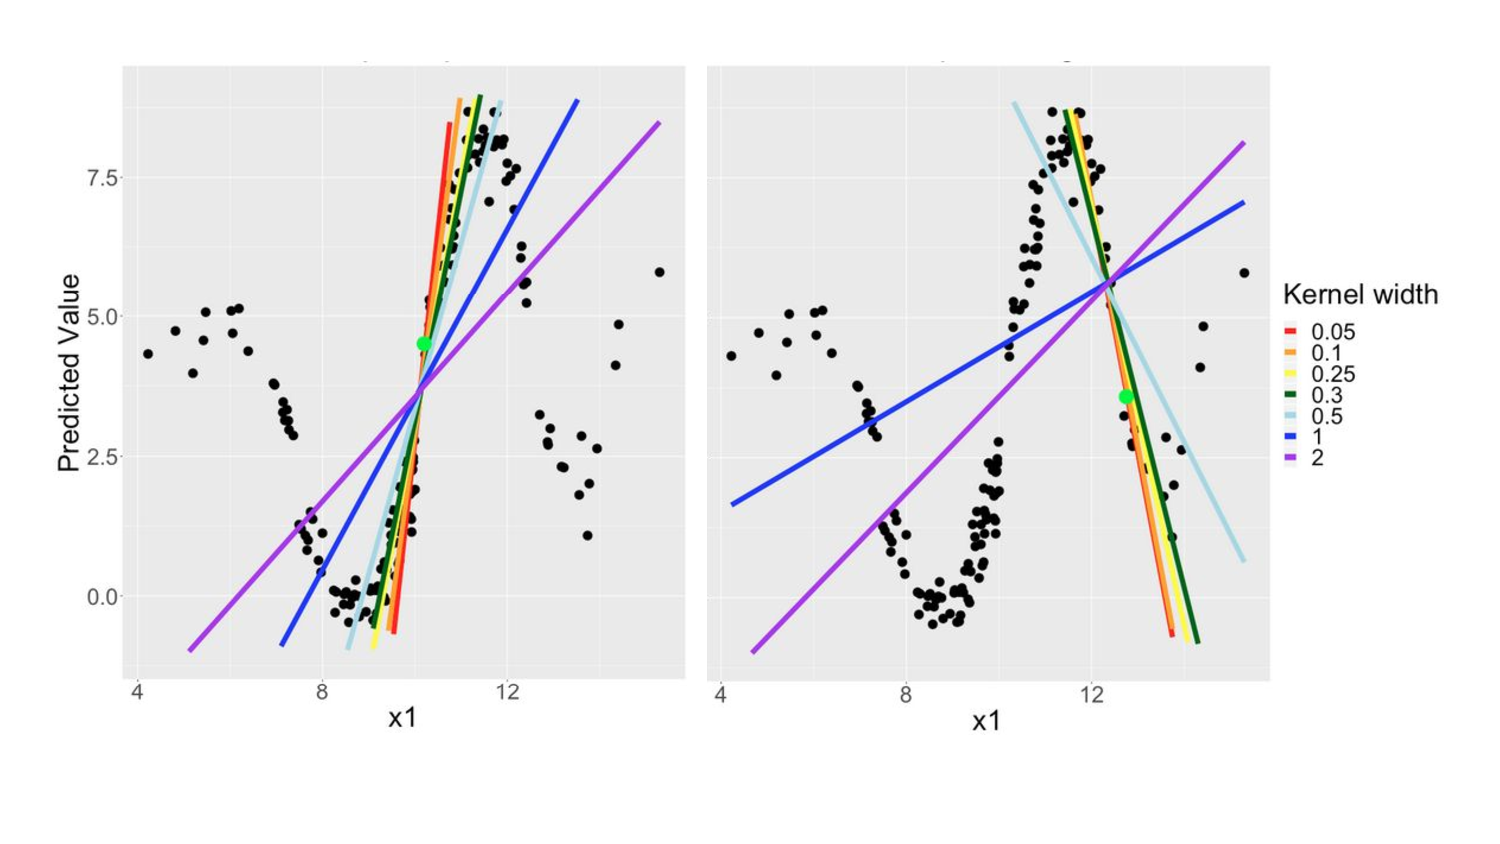
\includegraphics[width=0.6\textwidth]{figure/lime_locality}
    %  		\vspace{-0.5cm}
     		
    %  		\scriptsize{Linear surrogate models for two observations based on the same model with one target and one feature. Each line displays one linear surrogate model with different kernel width. In the right figure, larger kernel sizes are more severe.}
     		
    %  	\end{center}
     \end{itemize}
     \pause
     \begin{columns}[T, totalwidth=\linewidth]
        \begin{column}{0.65\textwidth}
        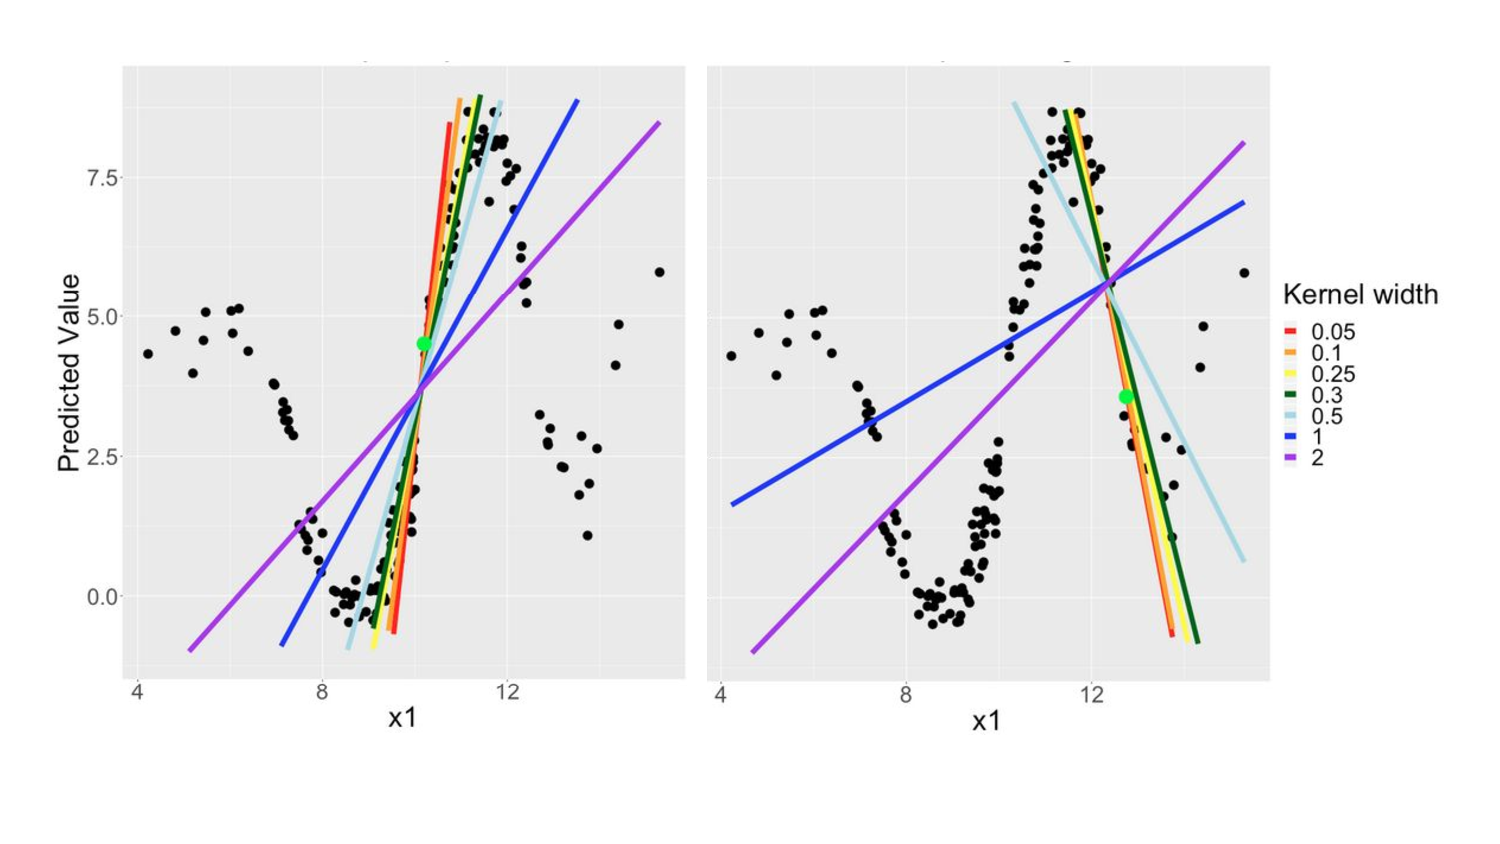
\includegraphics[width=\textwidth, trim = 0px 0px 30px 40px, clip]{figure/lime_locality}
         \end{column}
         \begin{column}{0.35\textwidth}
         \begin{itemize}
             \item Surrogate models for 2 obs. (green points) for same model with one feature $x_1$
             \item Each line refers to a linear surrogate model with different kernel width
             \item Right figure: larger kernel widths influence lines more
         \end{itemize}
         \end{column}
     \end{columns}
\end{frame}

\begin{frame}[c]{LIME Pitfall: Locality \citebutton{Kopper et al. 2019}{https://slds-lmu.github.io/iml_methods_limitations/}}
    \begin{itemize} 
         \item \textbf{Solution I}: Kernel width strongly interacts with locality:
         \begin{itemize}
             \item Large kernel width leads to interaction with points further away (unwanted)
             \item Small kernel width leads to small neighborhood\\
             $\leadsto$ risk of few data points\\
             $\leadsto$ potentially fitting more noise
         \end{itemize}
         \pause
    	\item \textbf{Solution II}: Use Gower distance where no kernel width needs to be specified 
    	\begin{itemize}
    	    \item \textbf{Problem}: data points far away receive weight $ > 0$\\
    	    $\leadsto$ resulting explanations are rather global than local surrogates   
    	\end{itemize}
    \end{itemize}
\vspace{0.3cm}

\end{frame}

\begin{frame}[c]{Pitfall: Local vs. Global Features \citebutton{Laugel et al. 2018}{https://arxiv.org/pdf/1806.07498.pdf}}

\begin{itemize}%[<+->]
	\item<1-> \textbf{Problem}: \\
	By sampling obs. for the surrogate model from the whole input space, the influence of local features might be hidden in favor of features with global influence (even for small kernel width)
	\item<2-> \textbf{Implication}: 
	\begin{itemize}
	    \item Some features influence the \textbf{global} shape of the black-box model
	    \item Other \textbf{local} features impact predictions only in smaller regions of $\Xspace$ %for a small area of $\Xspace$ 
	\end{itemize}
	\item<3-> \textbf{Example}: Decision trees\\
	$\Rightarrow$ Split features close to root have a more global influence than the ones close to leaves
\end{itemize}

\end{frame}


\begin{frame}{Pitfall: Local vs. Global Features -- Example \citebutton{Laugel et al. 2018}{https://arxiv.org/pdf/1806.07498.pdf}}

\begin{columns}
	\begin{column}{0.6\textwidth}
		\begin{itemize}
		\item Binary classification model
		\item Right figure: %Given in figure to the right:
		\begin{itemize}
		    \item Black and grey crosses: training data
		    \item Green dot: Obs. to be explained
		    \item Background color: Classification of random forest
		    \item Dark grey curve: Classifier's decision boundary
		    \item Dotted lines: Local decision boundary
		\end{itemize}
		\item \textbf{Observation:} Decision boundaries of LIME with different kernels (blue and green lines) do not match the direction of the local decision boundary\\ (which appears steeper)
	\end{itemize}
\end{column}
\begin{column}{0.39\textwidth}
%\vspace{0.3cm}

	\begin{center}
	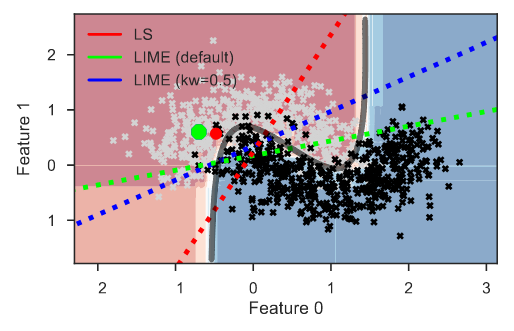
\includegraphics[width=1\textwidth]{figure/lime-globallocal2}

	{Half-moons dataset}
	
\end{center}

	\end{column}
\end{columns}
%\footnote[frame]{Laugel et al. (2018). Defining Locality for Surrogates in Post-hoc Interpretability. \url{https://arxiv.org/pdf/1806.07498.pdf}.}
\end{frame}

\begin{frame}{Pitfall: Local vs. Global Features -- Solution \citebutton{Laugel et al. 2018}{https://arxiv.org/pdf/1806.07498.pdf}}
\begin{columns}[T, totalwidth=\textwidth]
	\begin{column}{0.6\textwidth}
	%\vspace{-.5cm}
		\begin{itemize}
		\item \textbf{Solution}: 
		Find closest point to $\xv$ from other class and sample new points $\zv$ around it for higher local accuracy
		\begin{center}
		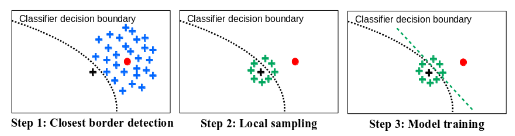
\includegraphics[width=\linewidth]{figure/laugel_method}
		\scriptsize{\textbf{Example:} $\xv$ (red point), closest point from other class (black cross)}
	    %{Local surrogate (LS) method by \citebutton{Laugel et al. 2018}{https://arxiv.org/pdf/1806.07498.pdf}}
		\end{center}
		%Sample new instances $\zv$ around the decision boundary closest from point $\xv$ for higher local accuracy
		\pause
		\item Red dot (right figure): Closest point from other class

		\item Red line: Local surrogate (LS) method \citebutton{Laugel et al. 2018}{https://arxiv.org/pdf/1806.07498.pdf}\\
		$\leadsto$ better approximates the local direction of the decision boundary 
	\end{itemize}
% 	\begin{center}
% 		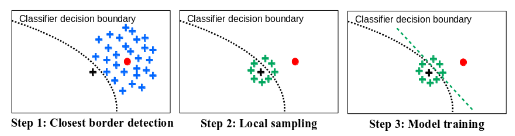
\includegraphics[width=1\textwidth]{figure/laugel_method}
% 	    {Local surrogate (LS) method by \citebutton{Laugel et al. 2018}{https://arxiv.org/pdf/1806.07498.pdf}}
% 		\vspace{-0.3cm}
% 		\end{center}
\end{column}
\begin{column}{0.39\textwidth}
%\vspace{0.3cm}

	\begin{center}
	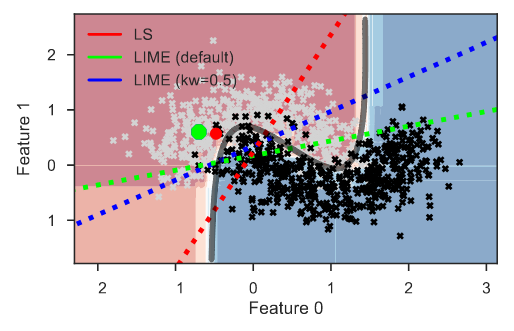
\includegraphics[width=1\textwidth]{figure/lime-globallocal2}
	
	{Half-moons dataset}
	
\end{center}

	\end{column}

\end{columns}
%\footnote[frame]{Laugel et al. (2018). Defining Locality for Surrogates in Post-hoc Interpretability. \url{https://arxiv.org/pdf/1806.07498.pdf}.}
\end{frame}


\begin{frame}[c]{Pitfall: Faithfulness}
\begin{itemize}
%\itemsep1em
	\item \textbf{Problem}: Trade-off between local fidelity vs. sparsity
	\item \textbf{Observation I}: Low fidelity $\leadsto$ unreliable explanations
	\item \textbf{Observation II}: High fidelity requires complex models $\leadsto$ difficult to interpret surrogate model %surrogate model cannot easily be interpreted
	\pause
	\item \textbf{Example: Credit data} 
	\begin{itemize}
	\itemsep0em
	    \item Original prediction by random forest for one data point $\xv$: 
	    $$\fh(\xv) = \hat{\P}(y = 1 ~|~ \xv) = 0.143$$
	    \item %Regularized linear model with only three selected features (\code{sex}, \code{checking.account}, \code{duration}) $g_{lm}(\xv) = 0.283$
	    Linear model with only three selected features (\code{age}, \code{checking.account}, \code{duration}):
	    $$g_{lm}(\xv) = \betah_0 + \betah_1 x_{age} + \betah_2 x_{checking.account} + \betah_3 x_{duration} = 0.283$$
	    \item Generalized additive model (with all 9 features) is more complex:
    $$%\begin{equation*} 
    %\begin{split}
    g_{gam}(\xv) = \betah_0 + f_{age}(x_{age}) + f_{checking.account}(x_{checking.account}) + f_{duration}(x_{duration}) +  \dots %& = \betah_0 + s_{age}(x_{age}) +s_{credit.amount}(x_{credit.amount}) s_{duration}(x_{duration}) + \betah_{sex = male} \ind_{sex = male}   \\
    %& + \betah_{job}(x_{job}) + \betah_{housing = own} \ind_{housing = own} +   \betah_{housing = rent} \ind_{housing = rent} \\
    %& + \betah_{saving.accounts = moderate} \ind_{saving.accounts = moderate} + \betah_{saving.accounts = rich} \ind_{saving.accounts = rich} \\
    %& + ... + \betah_{purpose = radio/TV} \ind_{purpose = radio/TV}  
    = 0.148$$
    %\end{split}
    %\end{equation*}
	\end{itemize}
\end{itemize}

\end{frame}

\begin{frame}{Pitfall: Hiding biases \citebutton{Slack et al. 2020}{https://arxiv.org/abs/1911.02508}}

\begin{itemize}
	\item \textbf{Problem}: Developer could manipulate their model to hide biases 
	\item \textbf{Observation}: LIME can sample out-of-distribution points (extrapolation)
	\pause
	\item \textbf{Attack} with adversarial model:
	    \begin{enumerate}
	    \item classifier to discriminate between in-distribution and out-of-distribution data points
	    \item for in-distribution points, use the original (biased) model
	    \item for out-of-distribution points produced for local explanation, use an unbiased model
	    \item[$\leadsto$] LIME samples out-of-distribution points and uses the unbiased model for local explanation\\
	    \item[$\leadsto$] this hides the bias of the true model
	    \end{enumerate}
\end{itemize}
	\begin{columns}[T, totalwidth=\linewidth]
		\begin{column}{0.5\textwidth}
	    \centering
	    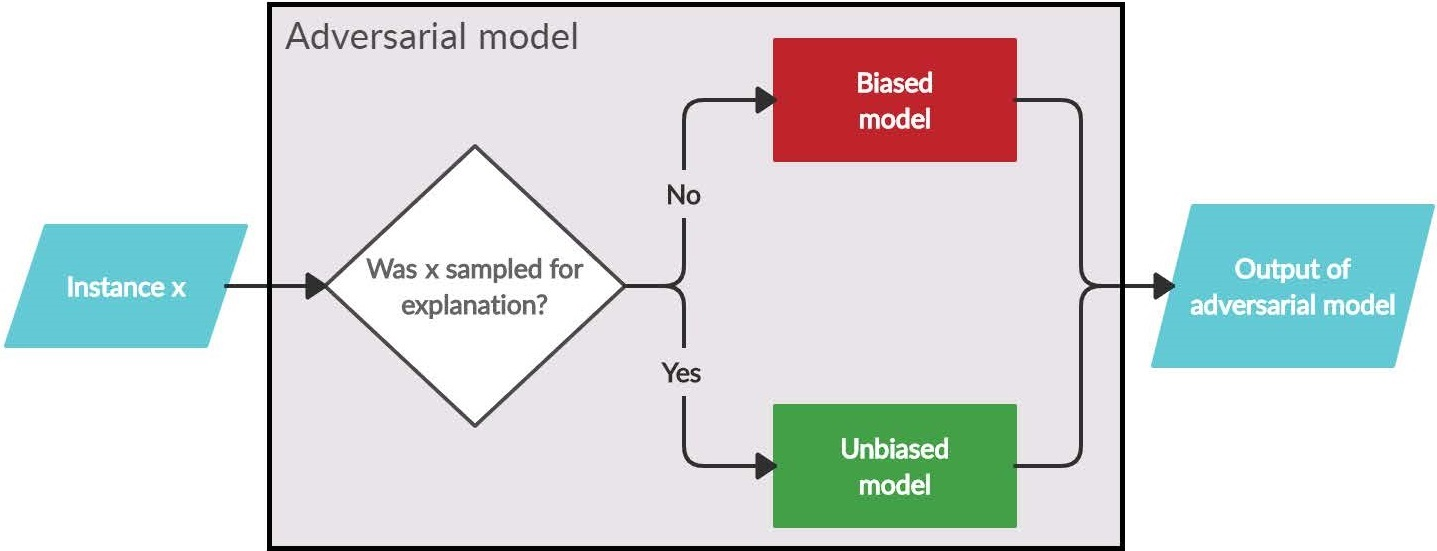
\includegraphics[width=\textwidth]{figure/attack_biased_unbiased.jpg}
	    \citebutton{Vres, Sikonja (2021)}{https://arxiv.org/abs/2101.11702}
	    \end{column}
\pause
	    \begin{column}{0.5\textwidth}
	    \textbf{Example}: Not using `gender` to approve a loan % Credit dataset %
	    \begin{itemize}
	        \item biased model trained on features correlated with `gender` (e.g. duration of parental leave)\\
	        $\leadsto$ used 
	        %for in-distribution points (realistic values) 
	        to make biased / unfair predictions
	        \item unbiased model trained on features uncorrelated with `gender`\\
	        $\leadsto$ used to produce explanations based on unbiased predictions to hide bias
	        %$\leadsto$ used for (extrapolated) LIME samples\\
	        %$\Rightarrow$ produced local explanations seem fair as they are based on unbiased model
	        %could be trained on features uncorrelated with `gender`
	    \end{itemize}
	    \end{column}
	\end{columns}
\end{frame}

\begin{frame}[c]{Pitfall: Robustness \citebutton{Alvarez-Melis, D., \& Jaakkola, T. 2018}{https://arxiv.org/abs/1806.08049}}
\begin{itemize}
	\item \textbf{Problem}: Instability of explanations 
	\item \textbf{Observation}: Explanations of two very close points could vary greatly 
	\begin{itemize}
	    \item[$\leadsto$] can happen because of other sampled data points $\zv$
	\end{itemize}
\end{itemize}
\vspace{-0.7cm}
\begin{columns}
	\begin{column}{0.48\textwidth}
		\begin{center}
		
		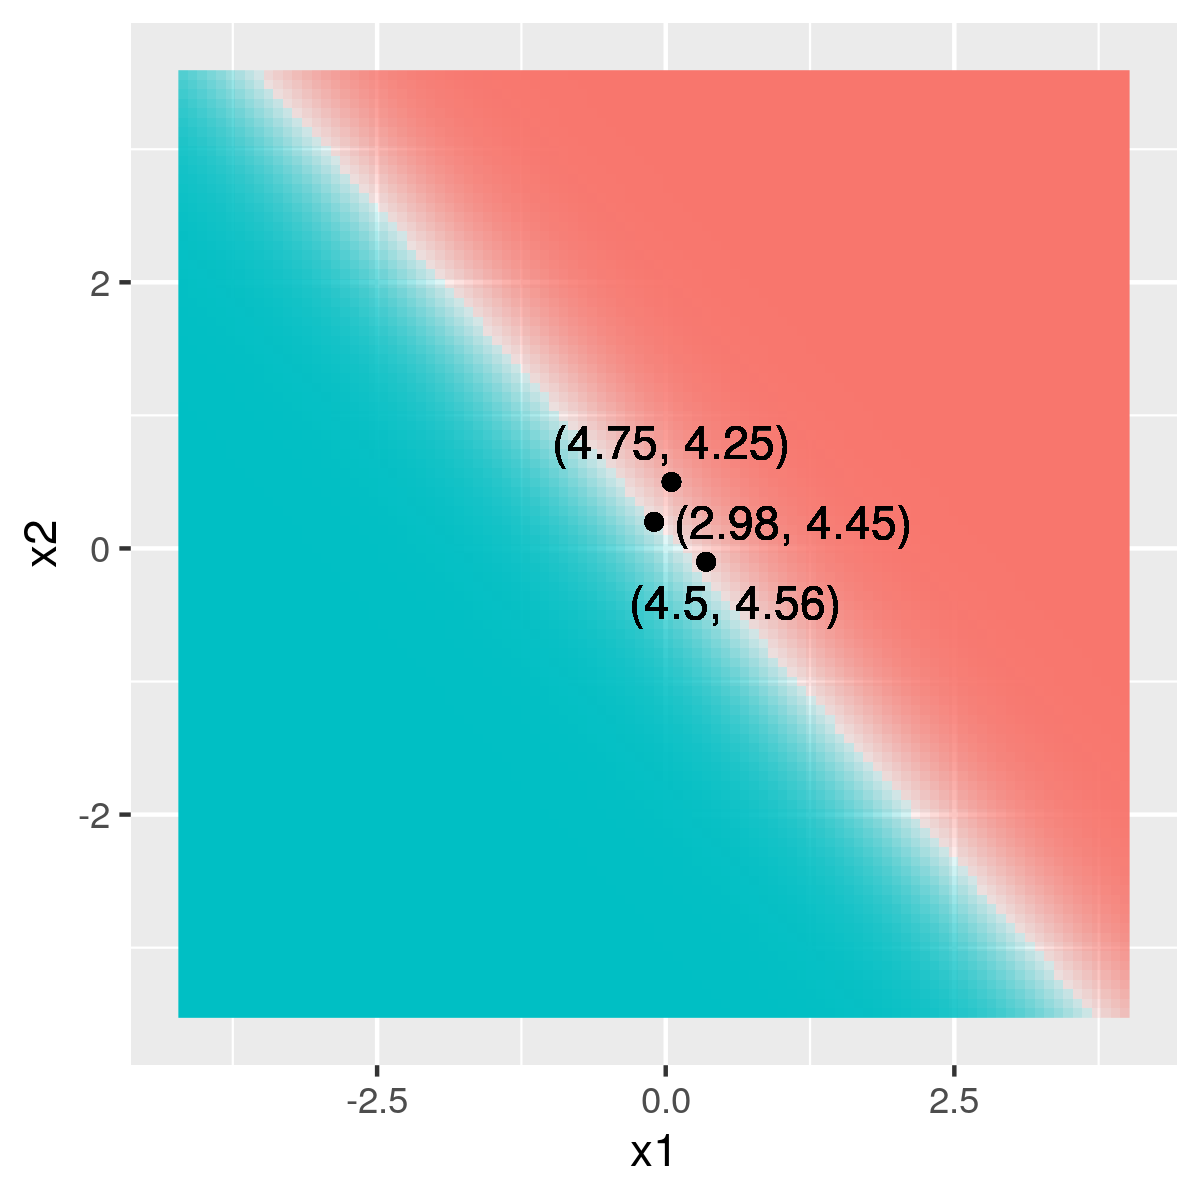
\includegraphics[width=0.55\textwidth]{figure/lime_robustness_1.png}
		
		{Linear prediction task (logistic regression). \\Linear surrogate returns similar coefficients for similar points.}
		
		\end{center}
	\end{column}
	\begin{column}{0.48\textwidth}
		\begin{center}
	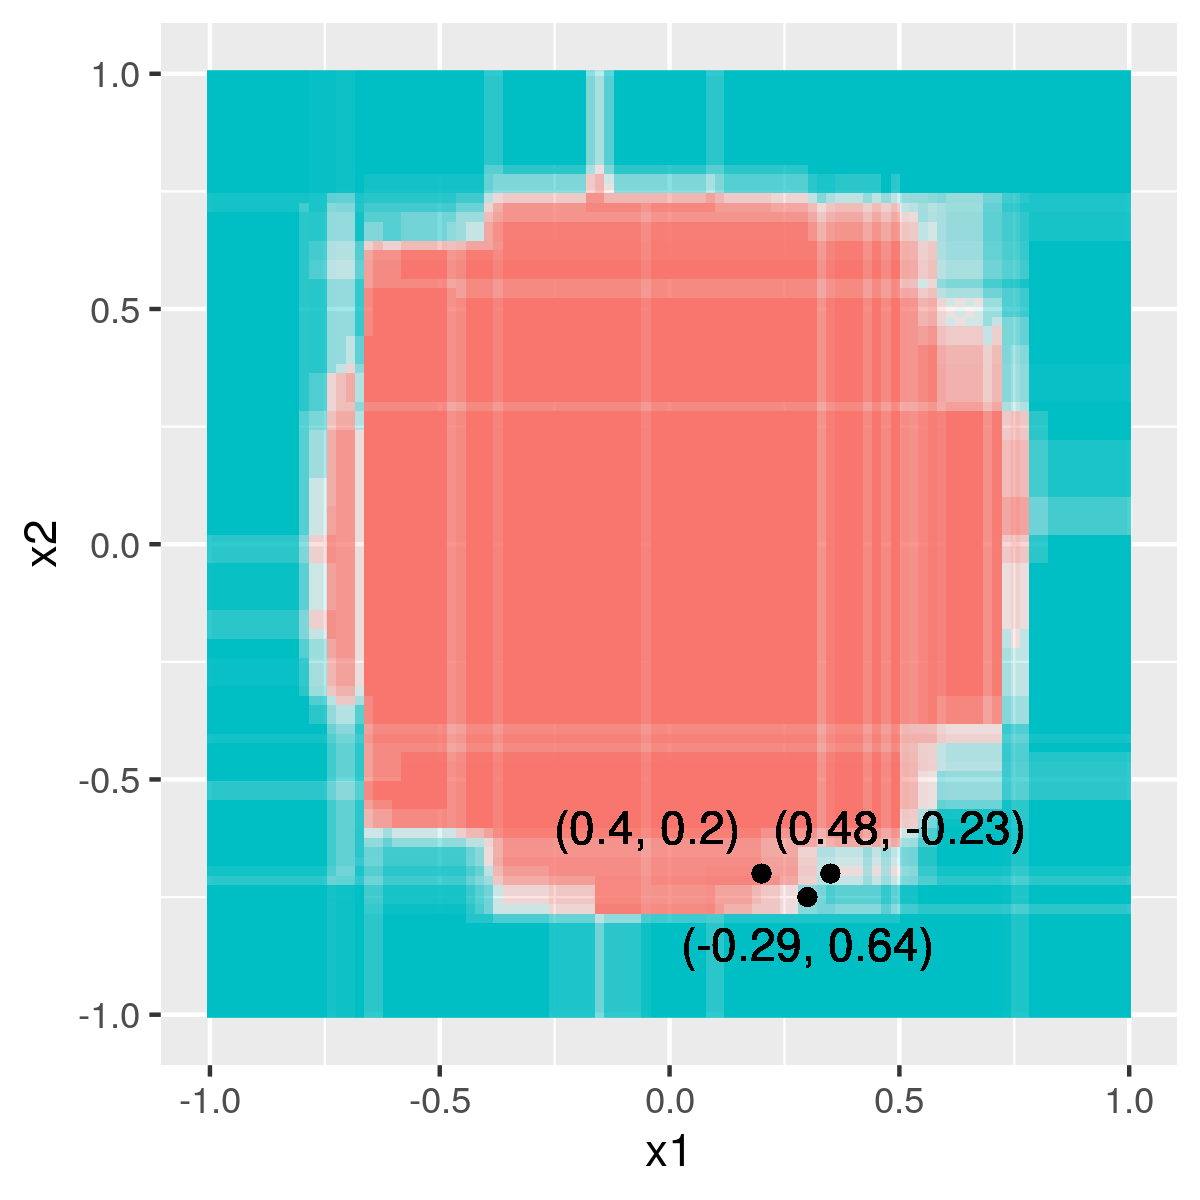
\includegraphics[width=0.55\textwidth]{figure/lime_robustness_2.png}
	
	{Circular prediction task (random forest). \\Linear surrogate returns different coefficients for similar points.}
	
	\end{center}
\end{column}
\end{columns}
\end{frame}

\begin{frame}{Pitfall: Definition of Superpixels \citebutton{Achanta et al. 2012}{https://ieeexplore.ieee.org/document/6205760}}

\begin{columns}
    
    \begin{column}{0.6\textwidth}
        
        \begin{itemize}
        	\item \textbf{Problem}: Instability because of specification of superpixels for image data 
        	\item \textbf{Observation}: Multiple specification of superpixels exist, influencing both the shape and size 
        	\pause
        	\item \textbf{Implication}: The specification of superpixel has a large influence on the explanations 
        	\item \textbf{Attack}: Change superpixels as part of an adversarial attack $\leadsto$ changed explanation
        \end{itemize}
        
    \end{column}
    
    \begin{column}{0.4\textwidth}
    
        \centering
        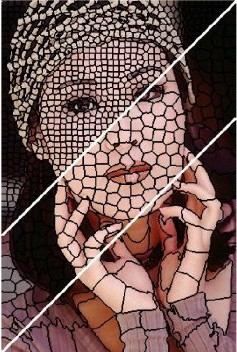
\includegraphics[width=0.7\textwidth]{figure/superpixel_woman}
        
    \end{column}
    
\end{columns}

\end{frame}


\endlecture
\end{document}